\documentclass{article}

\title{P6 Report}
\author{Nick Werle}

\usepackage{hyperref}
\usepackage{graphicx}

\begin{document}
\maketitle
\section{Preamble}
All necessary files will be uploaded to my githb repository at \url{https://github.com/NickWer/CEG3900_P6}

Additionally, as this is the halfway point submission, I have opted to make partial progress on each problem, rather than completing a few.
As a result, some of the work here will be more stream-of-conscious than my usual submissions. I plan to polish the report for the final deadline.

\section{Task 1}
I created four ubuntu server instances on AWS EC2 and then manually segmented each file into 13 rows (52 hashes to begin).
I let the four instances of John run for ~3 hours and managed, as expected to crack the guest password (guest007).

At this time I haven't started the android APK - it's unclear how I'm going to make it run.
That is, I think it won't be bad to start the process, but I'm unsure how I will be able to get the output/list collected passwords.
Perhaps two buttons - one that starts john, the other that runs `john --show etc-shadow-2009.txt` and returns that output.

	\begin{figure}[ht]
        \centerline{
            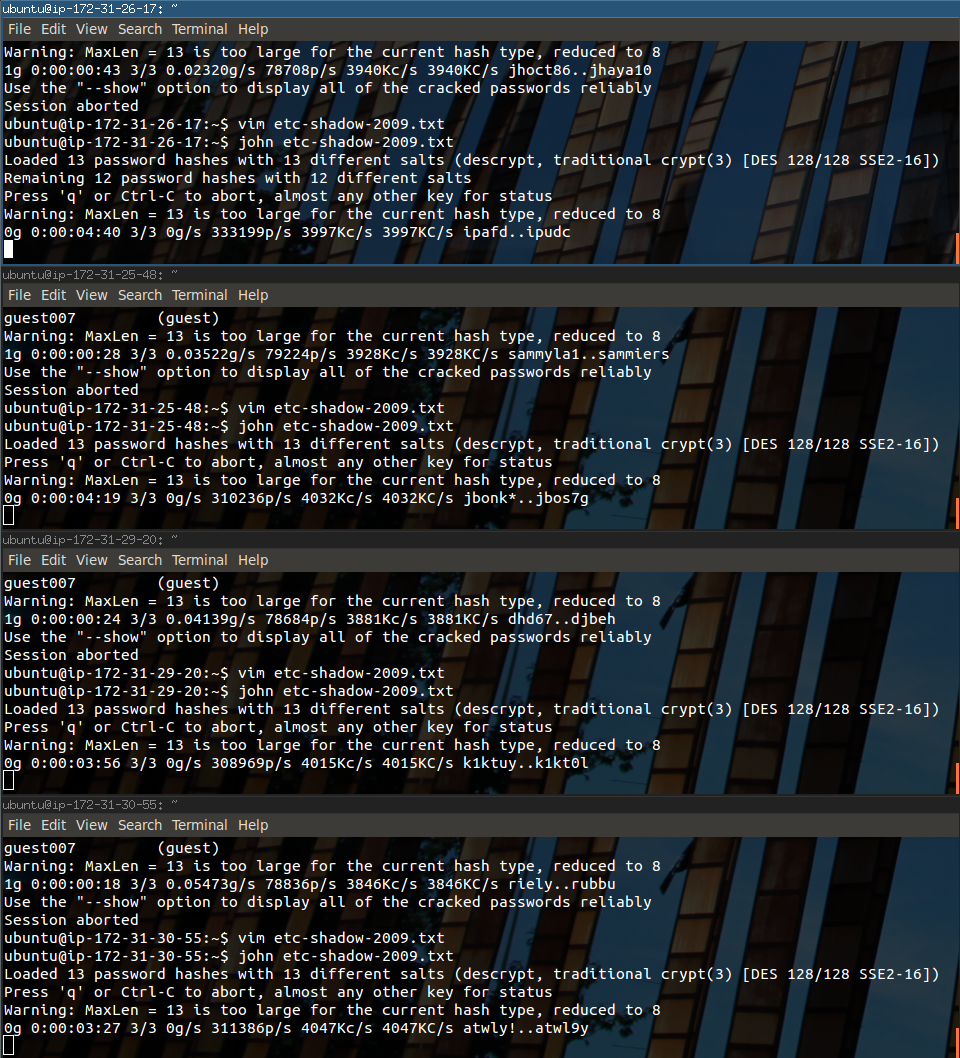
\includegraphics[width=7.5in]{img/t1s1.png}
        }
		\centering
		\caption{Task 1 - Four instances running at once over ssh}
	\end{figure}


\clearpage

\section{Task 2}
I was able to run hashcat on my desktop at home, which natively runs Ubuntu 16.04 (as opposed to my laptop that I `dist-uprade`ed to 16.04), and also includes an NVidia GPU as opposed to my laptop's AMD card.
I attempted to make a docker to see if it would run correctly inside of there, but it suffered from the same drivers issue that I struggled with before, and it didn't seem worth it to install those in the docker, too.
Anyways, I ran the hashcat program twice. Once with attack mode 0:

\begin{verbatim}
eb61eead90e3b899c6bcbe27ac581660:HELLO
2ac9cb7dc02b3c0083eb70898e549b63:Password1
75b71aa6842e450f12aca00fdf54c51d:P455w0rd
2c9341ca4cf3d87b9e4eb905d6a3ec45:Test1234
958152288f2d2303ae045cffc43a02cd:MYSECRET
eb61eead90e3b899c6bcbe27ac581660:HELLO
2ac9cb7dc02b3c0083eb70898e549b63:Password1
75b71aa6842e450f12aca00fdf54c51d:P455w0rd
2c9341ca4cf3d87b9e4eb905d6a3ec45:Test1234
958152288f2d2303ae045cffc43a02cd:MYSECRET
\end{verbatim}

Attack mode 3 (bruteforcing) was insanely slow, and I suspect would not have been able to find all of the passwords anyways, at least not today.
\begin{verbatim}
eb61eead90e3b899c6bcbe27ac581660:HELLO
2ac9cb7dc02b3c0083eb70898e549b63:Password1
75b71aa6842e450f12aca00fdf54c51d:P455w0rd
2c9341ca4cf3d87b9e4eb905d6a3ec45:Test1234
958152288f2d2303ae045cffc43a02cd:MYSECRET
\end{verbatim}

I have not yet completed the android APK

\section{Task 3}
I haven't technically started this yet, however I by creating the docker container for the previous section, I was able to trivially transfer my hashcat setup to the new machine.
To test it, I modified my dockerfile slightly from before:


\begin{verbatim}
FROM hihouhou/hashcat

ADD http://cecs.wright.edu/~pmateti/Courses/3900/Lectures/Assignments/hashes-md5.txt /root/
ADD http://downloads.skullsecurity.org/passwords/rockyou.txt.bz2

RUN apt-get install -y bzip2
RUN cd /root/ && bzip2 -d rockyou.txt.bz2
\end{verbatim}

and then the output:
\begin{verbatim}
[s]tatus [p]ause [r]esume [b]ypass [q]uit =>

Input.Mode: Dict (/root/rockyou.txt)
Index.....: 5/5 (segment), 553093 (words), 5720127 (bytes)
Recovered.: 5/8 hashes, 0/1 salts
Speed/sec.: 4.38M plains, 4.38M words
Progress..: 553093/553093 (100.00%)
Running...: 00:00:00:01
Estimated.: --:--:--:--


Started: Fri Apr  7 04:09:48 2017
Stopped: Fri Apr  7 04:09:53 2017
ubuntu@ip-172-31-26-17:~$
\end{verbatim}

The hashes cracked:
\begin{verbatim}
2ac9cb7dc02b3c0083eb70898e549b63:Password1
eb61eead90e3b899c6bcbe27ac581660:HELLO
75b71aa6842e450f12aca00fdf54c51d:P455w0rd
2c9341ca4cf3d87b9e4eb905d6a3ec45:Test1234
958152288f2d2303ae045cffc43a02cd:MYSECRET
\end{verbatim}

Finally, I found this article \url{http://blog.trifork.com/2013/12/24/docker-from-a-distance-the-remote-api/}. It appears that using this, I can trivially implement these android applications by just having the buttons send AJAX.
Full documentation is here: \url{https://docs.docker.com/engine/api/v1.27/}

One possible solution is to implement the UI as an ultra simple embedded web application, to streamline the interaction with the API (no need to worry about how to use the JSON objects).
That said, gson or something similar may be able to make use of it easily enough. I've used it before so it shouldn't be bad.

\section{Task 4}
I feel like I am very close - I am just really struggling to get cassandra to start from inside the docker, and not having much luck with linking an outside docker to this one.

Here is the post I made in pilot:
\begin{verbatim}


Trying to construct a docker image for painbow. Should I run a second docker for cassandra and link it to the painbow instance as they do in the docs at https://hub.docker.com/_/cassandra/ ?

Or should I run cassandra inside of my painbow docker - which is what I'm currently trying to do after giving up on the previous?

I get the following error:

nick@nick-lenovo ~/D/C/P/Task4> docker run -i nick/task4 bin/painbow --migrate
SLF4J: Failed to load class "org.slf4j.impl.StaticLoggerBinder".
SLF4J: Defaulting to no-operation (NOP) logger implementation
SLF4J: See http://www.slf4j.org/codes.html#StaticLoggerBinder for further details.
Exception in thread "main" com.datastax.driver.core.exceptions.NoHostAvailableException: All host(s) tried for query failed (tried: /127.0.0.1:9042 (com.datastax.driver.core.TransportException: [/127.0.0.1:9042] Cannot connect))
    at com.datastax.driver.core.ControlConnection.reconnectInternal(ControlConnection.java:227)
    at com.datastax.driver.core.ControlConnection.connect(ControlConnection.java:82)
    at com.datastax.driver.core.Cluster$Manager.init(Cluster.java:1307)
    at com.datastax.driver.core.Cluster.init(Cluster.java:159)
    at com.datastax.driver.core.Cluster.connect(Cluster.java:249)
    at us.yellosoft.painbow.Painbow.main(Painbow.java:154)

Basically: I'm unable to start cassandra within my docker.

Running `service cassandra start` outputs an error, too. Based on preliminary research this is expected when inside of a docker (security reasons) and non-fatal, but i'm not conviced.

docker run -i nick/task4 service cassandra start
/etc/init.d/cassandra: 72: ulimit: error setting limit (Operation not permitted)

Taking any and all ideas.

My dockerfile is basically a merge of the gradle and cassandra dockerfiles, plus RUN statements to build painbow.
\end{verbatim}

\end{document}
